\scanpage{83}

\deleted{\unsure{approcher} $(\rho_i)(\sigma_i)$ par les systèmes $(\rho'_i)=(\unsure{\rho_i})$, $(\sigma_i+\varepsilon)$ \inserted{\deleted{$(\sigma'_i)=$}} \illegible{1} du \unsure{même} \illegible{1} \unsure{pour} $k=\unsure{n}$, $\rho'_i,\sigma'_i$ qui satisfont encore aux conditions \unsure{énumérées} \unsure{sauf} que $\sigma'_{n-1}\ne0$ (en \unsure{prenant|posant}}

Il suffit donc, dans le cas \deleted{\unsure{général}}\inserted{\unsure{$\sigma_n=0$|\deleted{$\sigma_n=0$}}}, \unsure{\deleted{d'approcher}|d'approcher|\deleted{d'associer}} \inserted{d'approcher} $(\rho_i)$ $(\sigma_i)$ par un \inserted{système admissible} $(\rho'_i),(\sigma'_i)$ avec $\sigma_n>0$, et on prendra \deleted{$\unsure{\rho'_i=\rho_i}$}

\deleted{\deleted{\unsure{évidemment}} \unsure{l'inégalité|simplement|supposons} par des $(\rho'_i),(\sigma'_i)$, avec $\sigma'_{n-1}>0$, comme on voit en posant $(\rho'_i)=(\rho_i)$, $\sigma_i=\sigma'_i+\varepsilon$ pour \deleted{tout} $i\leq n-1$, $\sigma'_n=\sigma_n$ (on aura un système admissible, en particulier $\prod\rho'_i=\prod\sigma'_i=0$), ce qui nous ramène au cas où $\unsure{\sigma}_{n-1}>0$, $\sigma_n=0$. \deleted{\unsure{et dont}}}

\deleted{Dans ce cas, si on prend $\sigma'_i=\sigma_i$ pour $i\leq n-1$, $\sigma'_n=\sigma_n+\varepsilon$, le système $(\rho_i),(\sigma'_i)$ est admissible, \inserted{pour $\varepsilon$ assez petit}, sauf que, dans le cas où on impose $\prod\rho_i=\prod\sigma_i$, on n'aura \deleted{\unsure{certainement|peut-être}} pas $\prod\rho_i=\prod\sigma'_i$. Mais en augmentant suffisamment peu les $\rho_i$ nuls, on obtient un système $(\rho'_i)$ tel qu'on ait encore \deleted{\unsure{et $\rho$}} $\rho'_1\mathord{-}\,\mathord{-}\rho'_q\leq\sigma'_1\mathord{-}\,\mathord{-}\sigma'_q$ pour $q=1,\mathord{-}n$, et \deleted{\unsure{même}}\inserted{par} augmentation éventuelle de $\rho'_n$ \deleted{\unsure{jusqu'à}}\inserted{$\rho''_n$}, \deleted{\unsure{on obtiendra|on obtient} $\rho'_1\mathord{.}\,\mathord{-}\rho'_{n-1}\rho''_n=\sigma'_1\mathord{-}\,\mathord{-}\sigma'_n$. \unsure{Ce système} $\rho'_n=$}}

simplement $\rho'_i=\rho_i$, $\sigma'_i=\sigma_i+\varepsilon$.

Prouvons maintenant le lemme. Il est bien connu qu'une \deleted{toute} fonction convexe \deleted{\unsure{$f$}} $\varphi$ sur $R^n$ est de la forme $\varphi=\operatorname*{Sup}_{\unsure{k|k\in K}}L_k$ où les $L_k$ sont des \deleted{\uline{\unsure{formes}}}\inserted{fonctions} \uline{linéaires} \inserted{affines} sur $R^n$ (\unsure{car|ça}. résulte du fait que la partie de $R^n\times R$ au dessus du graphe de $\varphi$ est convexe $\unsure{\div}$ par définition des fonctions convexes et \unsure{fermée|fermé} car $\varphi$ est continue, --- donc intersection de demi-espaces fermés, dont on constate aussitôt
\reversemarginpar
\margin{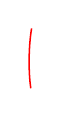
\begin{tikzpicture}[x=1cm,y=1cm]\draw[red,line width=.55pt] (0.02,0.76) .. controls (-0.02,0.52) and (-0.02,0.20) .. (0.01,0);\end{tikzpicture}}
\normalmarginpar
qu'ils \deleted{\unsure{ne peuvent} \unsure{avoir} pour} \textcolor{red}{\uline{\textcolor{black}{\inserted{peuvent} se mettre}}} \textcolor{red}{\uline{\textcolor{black}{sous la forme}}} \inserted{d'équations} $L_k(t)\geq0$).

De plus, si $\varphi$ est croissante, on voit \deleted{\unsure{qu'on} \illegible{2}}\inserted{que} les $L_k$ crois\unsure{santes}, i.e. \deleted{à coefficients} de la forme $L_k(t)=\sum_{i=1}^n a_it_i+\unsure{h|b}$, \deleted{\unsure{où les}}\inserted{avec} $a_i\geq0$ \inserted{pour \deleted{tout} $i$}. \deleted{Pour le voir,} : En effet, si on avait $a_i<0$, alors \deleted{la fonction} on

\reversemarginpar
\margin{84}
\normalmarginpar
